\chapter{Excel Neuron}
\section{Introduction}
Neural Networks, or more accurately artificial neural networks at their core a collection of simulated neurones. We can produce a simple neurone in Excel, that we can then get to learn a pattern and by repeating produce a simple neural network.

\section{Idea of a single artificial neuron}
At first, thinking about nerves and the brain may be at first a little scary - don't Panic. The neuron - the nerve cell - at basic level can be thought of a simple processing unit.

It has inputs these might be coming from other nerves or sensory input at this level we don't care really they are inputs and to start with the inputs are just going to be binary either 1 or 0. This is not as silly as it sounds in some nerves we either have the nerve firing (so a 1) or not firing (so a 0). This is simplistic but it a good starting point.
The neuron has an output again for all the examples in this chapter the output is going to be either 1 or 0.
The third part is the processing bit and this has two sub-parts. All the inputs are weighted, all this means is the particular input is multiplied to give a weighted value. As an example if the first input, let us call it X1 and it is 1, and the weight W1 is 0.1 then the weighted input is X1 x W1 =0.1. We do this for all the inputs and then we add all the weighted inputs together and produce a single number the weighted sum 0 first part done. The second part is taking the weighted sum and if the number is greater or equal to 0 then output is a 1 otherwise the output is 0.

One thing that we need to do is create a fake input X0=1 which is always 1 the weight W0 attached to it can change. For the moment please put up with this slightly strange thing - it is called a bias.

So, using figure 6.1 as our example
Weighted Sum = W0+W1.X1 +W2.X2 where . means times.
if Weighted Sum >=0 then Y(the output) =1 otherwise Y=0

So in the figure 6.1 example Weighted Sum = -1+X1+X2 (remember X1 and X2 can be 1 or 0). So to get an output (Y) to be 0 both X1 and X2 need to be 0 if one of then is a 1 then the output (y) is a 1. This is an OR gate. If we changed W0 from -1 to -2 then both X1 and X2 need to 1 to get a Y=1 - this is an AND gate.

The Big SEcret: Change the weights we can get different functions from the 'neurone'.

\begin{figure}
    \centering
    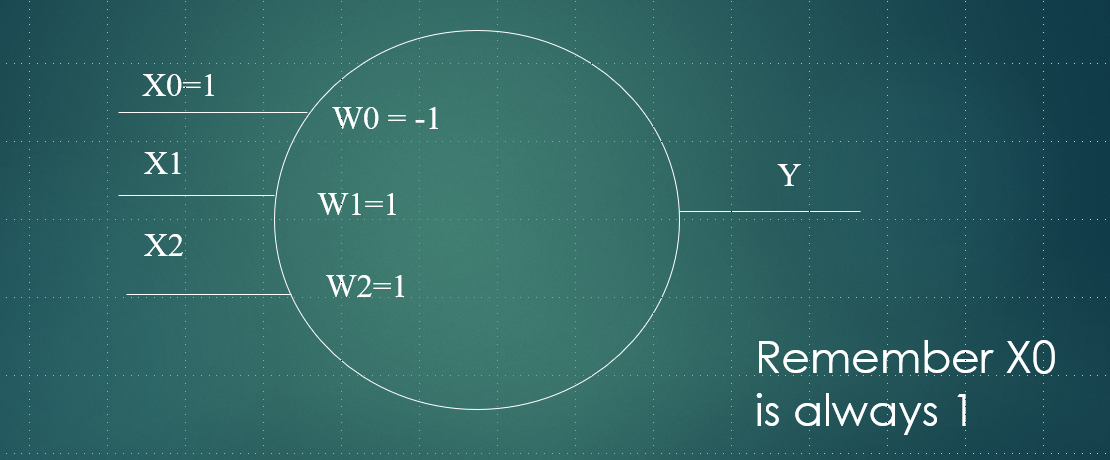
\includegraphics[width=10cm]{chapters/chAi1/figures/overall neurone2.png}
    \caption{Basic Artificial Neuron}
    \label{fig:basicneuron}
\end{figure}

\section{Building a Single Neuron}

On a blank sheet in either Excel or equivalent. 

1.  Write following headings 
A                B                            D                 E                 F                                      H                             J
X1	X2	 	W0	W1	W2	 	net 	 	Y

2.  Under X1 and X2 write down the four binary combinations - these are your inputs 

3   Under W0 W1 W2 write down three number W0 is the bias , W1 is the weight on input 1 and W2 is the weight on input 2

4 Under net on line 2 write this formula  =A2*$E$2+B2*$F$2+D2 and then copy and paste it into the next three cells below it.

5. Under Y type in the following  =IF(H2>=0,1,0)  and then copy and paste the formula to the three cells below it.


Hopefully it look similar to the one below.

X1	X2	 	W0	W1	W2	 	net 	 	Y

0	0	 	-2	1	1	 	-2	 	0

0	1	 	 	 	 	 	-1	 	0

1	0	 	 	 	 	 	-1	 	0

1	1	 	 	 	 	 	0	 	1


Questions

1 What logic operation has been carried out above?

2.If W0=1 W1=-1 and W2=-1  what logic operation do we have?

3. If W0=-1 W1=0 and W2=1  in terms of logic operation how else can be described Y in terms of X1 X2

4. Adjust the value of W0 (the bias) and then discuss with a colleague what do you think the main job of the bias is?

\section{Training a single neurone}

\section{Three neurones connect - we have a network}